% !TeX spellcheck = <none>
% Cheat sheet for probability theory and mathematical statistics
% By Vopaaz
\documentclass{article}
\usepackage{geometry}
\geometry{a4paper, top = 0.25 cm, bottom = 0.25 cm, left = 0.2 cm, right = 0.2 cm}
\usepackage{setspace}
\usepackage{enumerate}
\usepackage{enumitem}
\setenumerate[1]{itemsep=0pt,partopsep=0pt,parsep=0pt ,topsep=0pt}
\setitemize[1]{itemsep=0pt,partopsep=0pt,parsep=0pt ,topsep=0pt}
\usepackage{amsmath}
\usepackage{amssymb}
\usepackage{framed}
\usepackage{color}

\usepackage{verbatim}
\usepackage{multirow}
\usepackage{fontspec}
\usepackage[lining]{ebgaramond}

\usepackage{array}

\newcommand{\sectionline}{\color{black}\rule[2pt]{0.45\textwidth}{0.05em}\color{black}}

\newcommand{\bigtitle}[1]{
	\noindent
	\textbf{#1}
}

\newcommand{\smalltitle}[1]{
	\noindent
	\textbf{\textit{#1}}
}

\newcommand{\properframed}[1]{
	{
		\centering
		\vspace{-2 ex}
		\begin{framed}
			\vspace{-1.5 ex}
			#1
			\vspace{-1.5 ex}
		\end{framed}
		\vspace{-2 ex}
	}
}

%\usepackage{minted}
%\usemintedstyle{pastie}

\usepackage{tikz}
\usetikzlibrary{positioning,calc,shapes}

\begin{document}
\begin{spacing}{1.2}

\twocolumn

%-------%

\bigtitle{Laplace Transforms}

\smalltitle{General}

Definition: $F(s)=L[f(t)]=\int_{0}^{\infty} f(t) e^{-s t} d t$

Attribute: Linear Attribute

Differentiation: 

$\mathrm{L}\left[\dfrac{d f(t)}{d t}\right]=s F(s)-f(0)$

$\mathrm{L} \left[\dfrac{d^{n} f(t)}{d t^{n}}\right]=$

$s^{n} F(s)-\left[s^{n-1} f(0)+s^{n-2}\left.\dfrac{d f(t)}{d t}\right|_{t=0} +\ldots \ldots+\left.\dfrac{d^{n-1} f(t)}{d t^{n-1}}\right|_{t=0} \right]$

Integration: $\mathrm{L}\left[\int_{0}^{t} f(\tau) d \tau\right]=\dfrac{F(s)}{s}$

Initial / Final Value: 

$f(0)=\lim \limits_{s \rightarrow \infty} s F(s)$ 

$\lim \limits_{t \rightarrow \infty} f(t)=\lim \limits_{s \rightarrow 0} s F(s)$

Convolution: 

$f_{1}(t) \otimes f_{2}(t)=f_{2}(t) \otimes f_{1}(t)=\int_{0}^{t} f_{1}(t-\tau) f_{2}(\tau) d \tau$

$L\left[f_{1}(t) \otimes f_{2}(t)\right]=L\left[f_{1}(t)\right] L\left[f_{2}(t)\right]=F_{1}(s) F_{2}(s)$


\smalltitle{Inverse Laplace Transform}

Definition: [Not required] $f(t)=\mathrm{L}^{-1}[F(s)] =\dfrac{1}{2 \pi j} \int_{c-j \infty}^{c+j \infty} F(s) e^{s t} d \mathrm{s}$

Feasible methods:

If $F(s)=F_{1}(s)+F_{2}(s)+\ldots+F_{n}(s)$, then $f(t)=f_{1}(t)+f_{2}(t)+\ldots+f_{n}(t)$

If $F(s)=\dfrac{a_{0}+a_{1} s+\ldots+a_{m} s^{m}}{b_{0}+b_{1} s+\ldots+b_{n} s^{n}}$, then it can be break down to $F(s)=\dfrac{c_{1}}{\left(s-\lambda_{1}\right)}+\dfrac{c_{2}}{\left(s-\lambda_{2}\right)}+\cdots+\dfrac{c_{n}}{\left(s-\lambda_{n}\right)}$, where each item in this statement can be found in the Laplace table.

\smalltitle{Using Laplace Transform to differential equation}

\begin{enumerate}
\item Apply Laplace Transform to both sides on a differential equation.
\item Solve the Laplace equation.
\item Apply inverse Laplace Transform to the solution.
\end{enumerate}


\bigtitle{Transfer Function}

Definition: $G(s)=\dfrac{Y(s)}{U(s)}$, where $Y(s)$ is the Laplace Transform of the output $y(t)$ and $U(s)$ is that of the input $u(t)$.

Pole: Points that makes $G(s)$ go towards $\infty$.

For $\lim \limits_{s \rightarrow-p} G(s)(s+p)^{n}=C \neq 0 \quad n=1,2, \ldots$, we call $s=-p$ as the $n^{th}$ rank pole.

For $s=-r$ that makes $G(s) = 0$, it is a zero point. $r$ can be $\infty$.

Steps to get the transfer function of a system:

\begin{enumerate}
	\item Write down the differential equation of the system.
	\item Assume all the beginning values are zero, apply Laplace Transform.
	\item Get $\dfrac{Y(s)}{U(s)}$.
\end{enumerate}

\bigtitle{Close Ring System}

\begin{center}
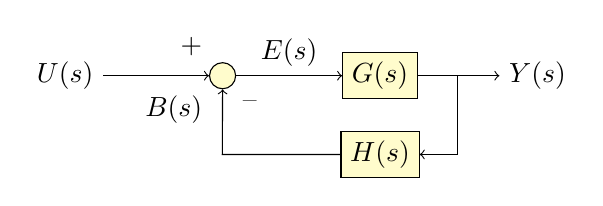
\begin{tikzpicture}[
process/.style={rectangle, draw, fill=yellow!20},
node distance=3cm
]
	\node at (0,0) (input) {$U(s)$};
	\node at (2,0) [circle, draw, fill=yellow!20] (adder) {};
	\node at (4,0) [process] (gs) {$G(s)$};
	\node at (6,0) (output) {$Y(s)$};
	\node [process] at (4,-1) (hs) {$H(s)$};
		
	\draw [->] (input) to (adder);
	\node [above left=0.5pt of adder] {+};
	
	\draw [->] (gs) to (output);
	\draw [->] ($(gs.east)+(0.5cm,0)$) -- ++(0,-1) -- ($(hs.east)$);
	
	\draw [->] ($(hs.west)$) -- ++(-1.5,0) -- (adder.south);
	
	\draw [->] (adder) to node [above] {$E(s)$} (gs);
	
	\node [below right=0.5pt of adder] {--};
	
	\node [below left=0.5pt of adder]{$B(s)$};
	
\end{tikzpicture}
\end{center}

Meaning of the figure:

$B(s)=H(s)Y(s)$

$Y(s)=E(s)G(s)$

$E(s)=U(s)-B(s)$

Every ``block"(Amplifier)'s output is the \textbf{product} of itself and \textbf{its input}.


Forward Transfer Function: $G_{F}(s)=\dfrac{Y(s)}{E(s)}=G(s)$

Open Ring Transfer Function: $G_{o}(s)=\dfrac{B(s)}{E(s)}=G(s) H(s)$

Close Ring Transfer Function $G_{C}(s)=\dfrac{Y(s)}{U(s)}=\dfrac{Y(s)}{E(s)+B(s)}$


\bigtitle{State Equation}

State variable: $x_i(t), i=1,2,\cdots,n$

State vector: $X(t)=\left[x_{1}(t) \quad x_{2}(t) \quad \cdots \quad x_{n}(t)\right]^{T}$


Standard description of a linear system:

Continuous:

$
\left\{
\begin{array}{l}
\dot{x}(t)=A(t) x(t)+B(t) u(t)\\
y(t)=C(t) x(t)
\end{array}
\right.
$

Discrete:

$
\left\{\begin{array}{l}{x(k+1)=A(k) x(k)+B(k) u(k)} \\ {y(k)=C(k) x(k)}\end{array}\right.
$

$A(t), B(t), C(t)$ or $A(k), B(k), C(k)$ can be constant $A,B,C$


\smalltitle{Defining the State Equation}

If the kinematic equation is $y^{(n)}+a_{n-1} y^{(n-1)}+\cdots+a_{1} \dot{y}+a_{0} y=u$

Let $x_{1}(t)=y(t), x_{2}(t)=\dot{y}(t), \cdots, x_{n}(t)=y^{(n-1)}(t)$

Then $
\left\{\begin{array}{l}{\dot{x}_{1}(t)=x_{2}(t)} \\ {\dot{x}_{2}(t)=x_{3}(t)} \\ {\vdots} \\ {\dot{x}_{n-1}(t)=x_{n}(t)} \\ {\dot{x}_{n}(t)=-a_{0} x_{1}(t) - \ldots -a_{n-1}x_{n}(t)+u(t)}\end{array}\right.
$

That is:

$
\dot{x}(t)=\left[ \begin{array}{ccccc}{0} & {1} & {0} & {\cdots} & {0} \\ {0} & {0} & {1} & {0} & {0} \\ {\vdots} & {\vdots} & {\vdots} & {\ddots} & {\vdots} \\ {0} & {0} & {0} & {\cdots} & {1} \\ {-a_{0}} & {-a_{1}} & {-a_{2}} & {\cdots} & {-a_{n-1}}\end{array}\right] x(t)+\left[ \begin{array}{c}{0} \\ {0} \\ {\vdots} \\ {0} \\ {1}\end{array}\right] u(t)
$

$y(t)=\left[ \begin{array}{lllll}{1} & {0} & {0} & {\cdots} & {0}\end{array}\right] x(t)$

\sectionline

If the kinematic equation is $y^{(n)}+a_{n-1} y^{(n-1)}+\cdots+a_{1} \dot{y}+a_{0} y=b_{m} u^{(m)}+\cdots+b_{1} \dot{u}+b_{0} u$

Apply Laplace Transform: 
$G(s)=\dfrac{Y(s)}{U(s)}=\dfrac{b_{m} s^{m}+\cdots+b_{1} s+b_{0}}{s^{n}+\cdots+a_{1} s+a_{0}}$

Let $Z(s)$ be an intermediate variable.

$\dfrac{Z(s)}{U(s)}=\dfrac{1}{s^{n}+\cdots+a_{1} s+a_{0}}$

$\dfrac{Y(s)}{Z(s)}=b_{m} s^{m}+\cdots+b_{1} s+b_{0}$

Eliminate the denominator and apple the Inverse Laplace Transform:

$z^{(n)}+a_{n-1} z^{(n-1)}+\cdots+a_{1} \dot{z}+a_{0} z=u$

$y=b_{m} z^{(m)}+b_{m-1} z^{(m-1)}+\cdots+b_{1} \dot{z}+b_{0} z$

[This can also be used to \textit{memorize} the place of $Z(s)$: $Z(s)$ should always combine with $\triangle s^{\triangle}$ after simplify the equation]

Choose $x_{1}(t)=z(t), x_{2}(t)=\dot{z}(t), \cdots, x_{n}(t)=z^{(n-1)}(t)$ as the state variable.

Then 

$
\left\{\begin{array}{l}{\dot{x}_{1}(t)=x_{2}(t)} \\ {\dot{x}_{2}(t)=x_{3}(t)} \\ {\vdots} \\ {\dot{x}_{n-1}(t)=x_{n}(t)} \\ {\dot{x}_{n}(t)=-a_{0} x_{1}(t)-\cdots-a_{n-1} x_{n}(t)+u(t)}\end{array}\right.
$

$y(t)=b_{0} x_{1}(t)+\cdots+b_{m} x_{m+1}(t)$

That is:

$\dot{x}(t)=\left[ \begin{array}{ccccc}{0} & {1} & {0} & {\cdots} & {0} \\ {0} & {0} & {1} & {0} & {0} \\ {\vdots} & {\vdots} & {\vdots} & {\ddots} & {\vdots} \\ {0} & {0} & {0} & {\cdots} & {1} \\ {-a_{0}} & {-a_{1}} & {-a_{2}} & {\cdots} & {-a_{n-1}}\end{array}\right] x(t)+\left[ \begin{array}{c}{0} \\ {0} \\ {\vdots} \\ {0} \\ {1}\end{array}\right] u(t)$

$y(t)=\left[ \begin{array}{cccccc}{b_{0}} & {\cdots} & {b_{m}} & {0} & {\cdots} & {0}\end{array}\right] x(t)$


\bigtitle{State Variable Graph}



\begin{minipage}{0.48\linewidth}
Integrator

\centering
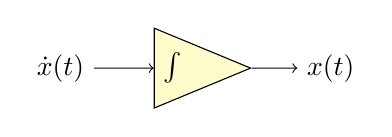
\begin{tikzpicture}
\node (in) at (0,0) {$\dot{x}(t)$};
\node [isosceles triangle, fill=yellow!20, draw] (int) at ($(in.east)+(1cm,0)$) {$\int$};
\node (out) at ($(int.east)+(1cm,0)$) {$x(t)$};

\draw[->] (in) to (int);
\draw[->] (int) to (out);
\end{tikzpicture}
\end{minipage}
\begin{minipage}{0.48\linewidth}
Delay

\centering

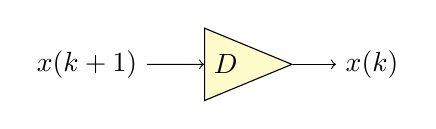
\begin{tikzpicture}
\node (in) at (0,0) {$x(k+1)$};
\node [isosceles triangle, fill=yellow!20, draw] (int) at ($(in.east)+(1cm,0)$) {$D$};
\node (out) at ($(int.east)+(1cm,0)$) {$x(k)$};

\draw[->] (in) to (int);
\draw[->] (int) to (out);
\end{tikzpicture}
\end{minipage}

For adder and amplifier, refer to \textbf{Close Ring System}.

\sectionline

\bigtitle{Acquiring Transfer Function from State Equation}

If the coefficient is constant:

$
\left\{\begin{array}{l}{\dot{x}(t)=A x(t)+B u(t)} \\ {y(t)=C x(t)}\end{array}\right.
$

Assume that the initial value of the system is zero, apply Laplace Transorm.

$s X(s)=A X(s)+B U(s)$

$Y(s)=C X(s)$

Recall that $G(s) = \dfrac{Y(s)}{U(s)}$, we can get:

\properframed{
$G(s)=C(I s-A)^{-1} B$.
}

\bigtitle{Acquiring State Equation from Transfer Function}

\smalltitle{Method 1.}

Firstly the original Transfer Function is:

$G(s)=\dfrac{Y(s)}{U(s)}=\dfrac{b_{m} s^{m}+\cdots+b_{1} s+b_{0}}{s^{n}+\cdots+a_{1} s+a_{0}}$

Let $V(s)$ be an intermediate function.

$\dfrac{Y(s)}{V(s)}=b_{m} s^{m}+\cdots+b_{1} s+b_{0}$

$\dfrac{V(s)}{U(s)}=\dfrac{1}{s^{n}+\cdots+a_{1} s+a_{0}}$

[Resembling \textit{Defining the state equation} part.]

Apply Inverse Laplace Transform,

let $x_i(t) = v^{(i-1)}(t), i=1,2,\ldots,n$:

$
\left\{\begin{array}{l}{\dot{x}_{1}(t)=x_{2}(t)} \\ {\dot{x}_{2}(t)=x_{3}(t)} \\ {\vdots} \\ {\dot{x}_{n-1}(t)=x_{n}(t)} \\ {\dot{x}_{n}(t)=-a_{0} x_{1}(t)-\cdots-a_{n-1} x_{n}(t)+u(t)} \\ \end{array}\right.
$

$y(t)=b_{0} x_{1}(t)+\cdots+b_{m} x_{m+1}(t)$

That is:

$\dot{x}(t)=\left[ \begin{array}{ccccc}{0} & {1} & {0} & {\cdots} & {0} \\ {0} & {0} & {1} & {0} & {0} \\ {\vdots} & {\vdots} & {\vdots} & {\ddots} & {\vdots} \\ {0} & {0} & {0} & {\cdots} & {1} \\ {-a_{0}} & {-a_{1}} & {-a_{2}} & {\cdots} & {-a_{n-1}}\end{array}\right] x(t)+\left[ \begin{array}{c}{0} \\ {0} \\ {\vdots} \\ {0} \\ {1}\end{array}\right] u(t)$

$y(t)=\left[ \begin{array}{cccccc}{b_{0}} & {\cdots} & {b_{m}} & {0} & {\cdots} & {0}\end{array}\right] x(t)$


\smalltitle{Method 2.}

Factorize $G(s)$

$\begin{aligned}
	G(s) & =\dfrac{b_{0}+b_{1} s+\ldots+b_{m} s^{m}}{a_{0}+a_{1} s+\ldots+s^{n}}                                                            \\
	     & =\dfrac{a_{0}+a_{1} s+\ldots+a_{m} s^{m}}{\left(s-\lambda_{1}\right)\left(s-\lambda_{2}\right) \cdots\left(s-\lambda_{n}\right)}
\end{aligned}$

If the denominator does not have multiple root:

$G(s)=\dfrac{c_{1}}{\left(s-\lambda_{1}\right)}+\dfrac{c_{2}}{\left(s-\lambda_{2}\right)}+\cdots+\dfrac{c_{n}}{\left(s-\lambda_{n}\right)}$,
where $c_i$ can be derived by fraction reduction.

Let:

$X_{1}(s)=\dfrac{1}{\left(s-\lambda_{1}\right)} U(s)$

$X_{2}(s)=\dfrac{1}{\left(s-\lambda_{2}\right)} U(s)$

$\cdots$

$X_{n}(s)=\dfrac{1}{\left(s-\lambda_{n}\right)} U(s)$

$Y(s)=c_{1} X_{1}(s)+c_{2} X_{2}(s)+\cdots+c_{n} X_{n}(s)$

Apply Inversed Laplace Transform,

$\dot{x}_{1}(t)=\lambda_{1} x_{1}(t)+u(t)$

$\dot{x}_{2}(t)=\lambda_{2} x_{2}(t)+u(t)$

$\cdots$

$\dot{x}_{n}(t)=\lambda_{n} x_{n}(t)+u(t)$

$y(t)=c_{1} x_{1}(t)+c_{2} x_{2}(t)+\cdots+c_{n} x_{n}(t)$

That is,

$
\left\{
\begin{array}{l}
	\dot{x}(t)=\left[ \begin{array}{ccc}{\lambda_{1}} & {\cdots} & {0}           \\
	{\vdots}                                          & {\ddots} & {\vdots}      \\
	{0}                                               & {\cdots} & {\lambda_{n}}
\end{array}\right] x(t)+\left[ \begin{array}{c}{1}
	         \\
	{\vdots} \\
	  {1}
\end{array}\right] u(t)\\
y(t) = \left[ c_1 \ \cdots \ c_n \right]x(t)
\end{array}
\right.
$


\sectionline

\bigtitle{State Transition Matrix for Discrete System}

Definition: $\Phi(k, l)=A(k-1) A(k-2) \cdots A(l+1) A(l) \quad k>l$

Attribute: 

$x(k)=\Phi(k, l) x(l) \quad k>l$

$\Phi(l, l)=I$

\bigtitle{Linear Discrete Free\footnote{$u(k)=0$} System}

Its state function is $x(k+1)=A(k) x(k)$

Then $x(k)=A(k-1) x(k-1)=A(k-1) A(k-2) \cdots A(1) A(0) x(0)$

Thus, $\Phi(k, l)=A(k-1) A(k-2) \cdots A(l+1) A(l) \quad k>l$

Let $x^1(k),\cdots, x^n(k)$ represent $n$ solutions to the state equation, which means that
$x^i(k+1) = A(k)x^i(k)$ holds true for all $k$.

If all $x^i(k)$ are linearly independent,

$X(k)=\left[x^{1}(k) \quad x^{2}(k) \quad \cdots \quad x^{n}(k)\right]$ is called Fundamental Solution Matrix.

Generally, $\Phi(k, l)=X(k) X^{-1}(l) \quad k>l$

\smalltitle{Deriving $\Phi(k,0)$ from State Equation}

Assume $x^i(0)$ are $n$ solutions for the State Equation.

Iterate $x^i(k+1) = A(k)x^i(k)$ to find the pattern (or expression) for $x^i(k)$.

Then, $X(k) = \left[ x^1(k) \quad x^2(k) \quad \ldots \quad x^n(k) \right]$.

And $X(0) = \left[ x^1(0) \quad x^2(0) \quad \ldots \quad x^n(0) \right] $.

$\Phi(k,0) = X(k) X^{-1}(0)$ [\textbf{Formula}]

Usually, let $X(0)$ be $I$, then $X^{-1}(0)$ is $I$ as well, which simplifies the calculation.

\sectionline

If $A$ is \textit{constant}:
$\Phi(k, l)=A^{k-l} \quad k \geq l$,

so $\Phi(k, 0)=A^{k} \quad k \geq 0$

Methods of calculating $A^k$:

\begin{enumerate}
	\item $A^{k}=(I+B)^{k}=I^{k}+\left( \begin{array}{c}{k} \\ {1}\end{array}\right) I^{k-1} B+\left( \begin{array}{l}{k} \\ {2}\end{array}\right) I^{k-2} B^{2}+\cdots+B^{k}$, where $\left( \begin{array}{c}{k} \\ {i}\end{array}\right)=\dfrac{k !}{(k-i) ! i !}$ and $B^k$ is easy to obtain
	\item Diagonalize $A = PBP^{-1}$, then $A^{k} = PB^kP^{-1}$
\end{enumerate}

\bigtitle{Linear Discrete System with $B(k)u(k)$}

Solution for $x(k+1)=A(k) x(k)+B(k) u(k)$ is:

\properframed{
$x(k)=\Phi(k,0)x(0) + \sum \limits_{l=0}^{k-1}\Phi(k,l+1)B(l)u(l)$
}

To obtain $\Phi(k,0)$, simply ignore $B(k)u(k)$ and apply the methods in \textit{Deriving $\Phi(k,0)$ from State Equation}.

\bigtitle{State Transition Matrix for Continuous System}

Definition: $x(t)=\Phi(t, \tau) x(\tau)$

Attribute:

$\dot{x}(t)=A(t) \Phi(t, \tau) x(\tau)$

$\dfrac{d \Phi(t, \tau)}{d t}=A(t) \Phi(t, \tau)$

$\Phi(\tau, \tau)=I$

$\Phi\left(t_{2}, t_{0}\right)=\Phi\left(t_{2}, t_{1}\right) \Phi\left(t_{1}, t_{0}\right)$

$\Phi\left(t_{1}, t_{0}\right)=\Phi^{-1}\left(t_{0}, t_{1}\right)$


\bigtitle{Linear Continuous Free System}

Let $x^1(k),\cdots, x^n(k)$ represent $n$ solutions to the state equation, which means that

$X(t) = \left[ x^1(t) \quad x^2(t) \quad \ldots \quad x^n(t) \right]$ satisfies $\dot{X}(t)=A(t) X(t)$

Then, $\Phi(t, \tau)=X(t) X^{-1}(\tau)$

\smalltitle{Constant $A$}

It can be derived that 

$x(t) = \left( I+At+\dfrac{1}{2}A^2t^2 + \cdots + \dfrac{1}{k!}A^kt^k + \cdots \right) x(0)= e^{At}x(0)$

That is,
$\Phi(t,0) = e^{At}$

$\Phi(t, \tau)=e^{A t} e^{-A \tau}=e^{A(t-\tau)}$

\bigtitle{Computing $e^{At}$}

If $A$ is diagonal:

$A=\left[ \begin{array}{cccc}{a_{1}} & {0} & {\dots} & {0} \\ {0} & {a_{2}} & {\dots} & {0} \\ {\vdots} & {\vdots} & {\ddots} & {\vdots} \\ {0} & {0} & {\dots} & {a_{n}}\end{array}\right]$

Then

$e^{A}=\left[ \begin{array}{cccc}{e^{a_{1}}} & {0} & {\cdots} & {0} \\ {0} & {e^{a_{2}}} & {\dots} & {0} \\ {\vdots} & {\vdots} & {\ddots} & {\vdots} \\ {0} & {0} & {\cdots} & {e^{a_{n}}}\end{array}\right]$

If $A$ is diagonalizable:

$A=P \Lambda P^{-1}$, where $\Lambda$ is diagonal, then $e^{A}=P e^{\Lambda} P^{-1}$.

If $A$ is not diagonalizable:

$A=P J P^{-1}$, where $J$ is the Jordan Standard Form.

Then use the definition:

$e^{At} = \left(I+A t+\dfrac{1}{2} A^{2} t^{2}+\cdots+\dfrac{1}{k !} A^{k} t^{k}+\cdots\right)$ 

and the \textbf{taylor series formula}.

$e^{x}=\sum \limits_{n=0}^{\infty} \dfrac{x^{n}}{n !}=1+x+\dfrac{x^{2}}{2 !}+\dfrac{x^{3}}{3 !}+\cdots$

About matrix diagonalization and Jordan Standard form, refer to other materials.


Or, recite this:

For $A=\left( \begin{array}{cccc}
\lambda &1&& \\
&\lambda&1& \\
&&\lambda&1\\
&&&\lambda
\end{array} \right)$

$A^k = \left(
\begin{array}{rrrr}
\lambda^k & k\lambda^{k-1} & \frac{k(k-1)}{2}\lambda^{k-2} & \frac{k(k-1)(k-2)}{6}\lambda^{k-3} \\
&\lambda^k & k\lambda^{k-1} & \frac{k(k-1)}{2}\lambda^{k-2}\\
&&\lambda^k & k\lambda^{k-1}\\
&&&\lambda^k
\end{array}
\right)$

$e^{At} = 
\left(
\begin{array}{rrrr}
e^{\lambda t} & t e^{\lambda t} & \frac{t^2}{2} e^{\lambda ^t } & \frac{t^3}{6} e^{\lambda^t} \\
&e^{\lambda t} & t e^{\lambda t} & \frac{t^2}{2} e^{\lambda ^t } \\
&&e^{\lambda t} & t e^{\lambda t}\\
&&&e^{\lambda t}
\end{array}
\right)
$




\bigtitle{Linear Continuous System with $B(t)u(t)$}

For $\dot{x}(t)=A(t) x(t)+B(t) u(t)$,

\properframed{
Solution is $x(t)=\Phi(t, 0) x(0)+\int_{0}^{t} \Phi(t, \tau) B(\tau) u(\tau) d \tau$
}

\bigtitle{Summary}

For
$x(k+1)=A x(k)+B u(k)$,
$\Phi(k, l)=A^{K-l}$

For
$\dot{x}(t)=A x(t)+B u(t)$,
$\Phi(t, \tau)=e^{A(t-\tau)}$


\sectionline

\bigtitle{Eigenvectors of a System}

For $x(k+1)=A x(k)$

The eigenvalues and eigenvectors are correspondingly:

$\lambda_{1}, \lambda_{2}, \ldots, \lambda_{n}$

$e_{1}, e_{2}, \ldots, e_{n}$

$\star$ If $x(0)=\alpha e_i$ ($\alpha$ here is a \textbf{scalar}), then 

$x(1)=A x(0)=A \alpha e_{i}=\lambda_{i} \alpha e_{i}=\lambda_{i} x(0)$

$x(2)=A x(1)=A \lambda_{i} \alpha e_{i}=\lambda_{i}^{2} \alpha e_{i}=\lambda_{i}^{2} x(0)$

$\cdots$

$x(k)=A x(k-1)=A \lambda_{i}^{k-1} \alpha e_{i}=\lambda_{i}^{k} \alpha e_{i}=\lambda_{i}^{k} x(0)$

[\textit{Mind that the $x(k)$ expressed like this are solutions to the differential function.}]

Let a variable $z(k)$ satisfy $x(k)=z(k)e_i$,
then $z_{i}(k+1)=\lambda_{i} z_{i}(k)$.

\bigtitle{Diagonalization of a Discrete System}

As the $e_i$ are linearly independent, any $x(k)$ can be expressed as 

$x(k)=z_{1}(k) e_{1}+z_{2}(k) e_{2}+\ldots+z_{n}(k) e_{n}$

It satisfies $x(k+1)=z_{1}(k+1) e_{1}+z_{2}(k+1) e_{2}+\ldots+z_{n}(k+1) e_{n}$

Also, $z_{i}(k+1)=\lambda_{i} z_{i}(k)$.

Let $x(k)=Mz(k)$ [\textbf{Formula}],

where $M=\left[ e_1 \quad \cdots \quad e_n \right]$,
$z(k)=\left[ \begin{array}{c}{z_{1}(k)} \\ {\vdots} \\ {z_{n}(k)}\end{array}\right]$

$x(k+1)=M z(k+1)=Ax(k)=A M z(k)$

$
\Rightarrow
z(k+1)=M^{-1} A M z(k)
$ [\textbf{Formula}]

It's easy to proof: $M^{-1} A M=\Lambda$,
$z(k+1)=\left[ \begin{array}{ccc}{\lambda_{1}} & {\cdots} & {0} \\ {\vdots} & {\ddots} & {\vdots} \\ {0} & {\cdots} & {\lambda_{n}}\end{array}\right] z(k)$


Also, $\Phi(k,0) = A^{k}=M \Lambda^{k} M^{-1}$ for constant $A$.


\bigtitle{Diagonalization of a Continuous System}

For $\dot{x}(t)=A x(t)$

The eigenvalues and eigenvectors are correspondingly:

$\lambda_{1}, \lambda_{2}, \ldots, \lambda_{n}$

$e_{1}, e_{2}, \ldots, e_{n}$

Let $\mathrm{M}=\left[e_{1}, e_{2}, \ldots, e_{n}\right]$ and $x(t)=M z(t)$

Then, $\dot{z}(t)=M^{-1} A M z(t)$

and $\dot{z}(t)=\left[ \begin{array}{ccc}{\lambda_{1}} & {\cdots} & {0} \\ {\vdots} & {\ddots} & {\vdots} \\ {0} & {\cdots} & {\lambda_{n}}\end{array}\right] z(t)$

Also, $\Phi(t,0) = e^{A t} =M e^{\Lambda t} M^{-1}$, and $e^{\Lambda t}=\left[ \begin{array}{ccc}{e^{\lambda_{1} t}} & {\dots} & {0} \\ {\vdots} & {\ddots} & {\vdots} \\ {0} & {\cdots} & {e^{\lambda_{n} t}}\end{array}\right]$



\bigtitle{Left Eigenvectors and Right Eigenvectors}

For $x(k+1)=A x(k)$,

Vector $f_i$ that satisfies $f_{j}^{T} A=\lambda_{j} f_{j}^{T}$ are the left eigenvectors of $A$, denoted as $f_{1}, f_{2}, \ldots, f_{n}$.

Attributes: 

$f_{i}^{T} e_{j}=0 \quad$ if $\quad i \neq j$

$f_{i}^{T} e_{i}=1$ (After it's standardized)

$f_i^T x(k) = z_i(k)$



\smalltitle{Multiple Eigenvalues}

If there are multiple eigenvalues for $A$, then it cannot be diagonalize. A can be transformed into Jordan Normal Form.


\bigtitle{Equilibrium Points}

Definition, a vector $\overline{x}$ that satisfies: once the system is $\overline{x}$, then the system will always be $\overline{x}$.

\smalltitle{Free System}

For both discrete and continuous free system,

$\overline{x} = 0$ is \textbf{always} a equilibrium point.


\smalltitle{Discrete Free System}

$x(k+1)=x(k)=\overline{x}$

That is, $\overline{x}=A \overline{x}$

As $A e=\lambda e$, so if any eigenvalue $\lambda=1$, its corresponding eigenvector $e$ is its equilibium point.

\smalltitle{Discrete System}

For $x(k+1)=A x(k)+b$,

$x(k+1)=x(k)=Ax(k)+b \Rightarrow \overline{x}=A \overline{x}+b$

That is, $(I-A) \overline{x}=b$, $\overline{x}=(I-A)^{-1} b$

If $(I-A)^{-1}$ does not exist, there is no equilibrium.

\smalltitle{Continuous Free System}

For $\dot{x}(t)=A x(t)$,

If a system is at its equilibrium, then its state does not change, $\dot{x}(t)=0$.

If $x(t)=e_{i}$ and this $e_i$'s corresponding $\lambda_i = 0$, 

then $\lambda_{i} x(t)=A x(t)=\dot{x}(t)=0$, which is an equilibrium.




\smalltitle{Continuous System}

For $\dot{x}(t)=A x(t)+b$

If a system is at its equilibrium, then its state does not change, $\dot{x}(t)=0$.

$0=A \overline{x}+b \Rightarrow \overline{x}=A^{-1} b$

If $A^{-1}$ does not exist, there is no equilibrium.



\bigtitle{Stability}

Definition: For any initial status, the state vector approaches the equilibrium as the time goes. Then the equilibrium is asymptotically stable.

\smalltitle{Convert Controlled System to Free System}

$x(k+1) - \overline{x} = A(x(k) - \overline{x})$

Let $z(k) = x(k) - \overline{x}$, $x(k+1)-\overline{x} \Rightarrow z(k+1) = Az(k)$

Thus, $x(k) \rightarrow \overline{x} \Leftrightarrow z(k) \rightarrow 0$, controlled system's approaching the equilibrium is equivalent to a free system, with the same $A$ matrix, approaching 0.

\smalltitle{Discrete System}

The equivalent condition of discrete system's asymptotically stability is all its $A$'s $|\lambda_i| < 1$. That is, the norm of all the eigenvalues are less than one, or all the eigenvalues are in the unit circle.

When the largest norm of all the eigenvectors is 1, if there is no multiple eigenvalue, it's called critical stable. If there are multiple eigenvalues, it's not stable.

\smalltitle{Continuous System}

The equivalent condition of continuous system's asymptotically stability is all its $A$'s $\operatorname{Re}(\lambda_i) < 0$. That is, the real part of all the eigenvalues are less than zero, or all the eigenvalues are to the left of the y-axis on the complex plane.

When the largest real part of all eigenvectors is 0, if there is no multiple eigenvalue, it's called critical stable. If there are multiple eigenvalues, it's not stable.

\smalltitle{Summary}

Linear constant system is asymptotically stable if:

Discrete System: All eigenvalues of $A$ are in the unit circle.

Continuous System: All eigenvalues of $A$ are in the left side of the complex panel.

\bigtitle{Oscillation}

\smalltitle{Discrete System}

Oscillate if there is imaginary or negative eigenvalue.

\smalltitle{Continuous System}

Oscillate if there is imaginary eigenvalue.


\bigtitle{Dominant Mode}

Defining the major behavior of the system in the long run.

\smalltitle{Discrete System}

The dominant eigenvalue is the $\lambda_1$ which has the largest norm.

$\lambda_{1} \& e_1$ is called the dominant mode.

The speed that the system converge to the equilibrium point is decided by $\lambda_1$.

If $\lambda_{1}$ is 1, the speed is decided by $\lambda_{2}$, whose norm is the second largest.

For discrete free system, there must be an eigenvalue = 1 (refer to ``Equilibrium Points - \textit{Discrete Free System}"), so its converging speed is decided by the second largest eigenvalue $\lambda_{2}$.

\smalltitle{Continuous System}

The dominant eigenvalue is the $\lambda_{1}$ which has the largest real part.

$\lambda_{1} \& e_1$ is called the dominant mode.

The speed that the system converge to the equilibrium point is decided by $\lambda_1$.

If $\lambda_{1}$ is 0, the speed is decided by $\lambda_{2}$, whose real part is the second largest.

For continuous free system, there must be an eigenvalue = 0 (refer to ``Equilibrium Points - \textit{Continuous Free System}"), so its converging speed is decided by $\lambda_{2}$.


\bigtitle{Positive Linear System}

Definition: The linear system whose state variable are always positive (or at least non-negative).

It is related to the positive matrix.

\smalltitle{Positive Matrix}

Definition:

Let $A = [a_{ij}]$ be a matrix,

\begin{itemize}
	\item If $\forall i,j, a_{ij} > 0$, $A$ is strictly positive, $A>0$
	\item If $\forall i,j, a_{ij} \geq 0$ and $\exists k,l, a_{kl} > 0$, $A$ is strictly non-negative or positive, $A\geq 0$
	\item If $\forall i,j, a_{ij} \geq 0$, $A$ is non-negative, $A \geqq 0$
\end{itemize}

Define:

\begin{itemize}
	\item $A \geq B \Leftrightarrow A-B \geq 0$
	\item $A>B \Leftrightarrow A-B>0$
	\item $A \geqq B \Leftrightarrow A-B \geqq 0$
\end{itemize}


\bigtitle{Frobenius-Perrion theorem}

\smalltitle{Theorem 1}

If $A>0$, then there exists such $\lambda_0 > 0$ and $X_0 > 0$, which:

\begin{itemize}
	\item $AX_0 = \lambda_0 X_0$
	\item For any other eigenvalue $\lambda \neq \lambda_0$, $|\lambda| < \lambda_0$. That is, $\lambda_0$ is the dominate eigenvalue
	\item $\lambda_0$ is a single eigenvalue (no duplication)
\end{itemize}

\smalltitle{Theorem 2}

If $A\geq 0$ and there exists such $m>0$ that $A^m > 0$, then Theorem 1 holds true.

\smalltitle{Theorem 3}

If $A\geqq 0$, there exists $\lambda_0 \geq 0$ and $X_0 \geq 0$ such that:

\begin{itemize}
	\item $AX_0 = \lambda_0 X_0$
	\item For any other eigenvalue $\lambda \neq \lambda_0$, $|\lambda| \leq \lambda_0$
\end{itemize}

Note that this theorem does not ensure $\lambda_0$ to be the single eigenvalue.

\smalltitle{The $\mathbf{\boldsymbol{\lambda}_0}$}

The above-mentioned $\lambda_0$ is called the Frobenius-Perron eigenvalue.

It can be estimated as follows:

Let $a_i$ be the sum of each row, then $\min(a_i) \leq \lambda_0 \leq \max(a_i)$

Let $b_i$ be the sum of each column, then $\min(b_i) \leq \lambda_0 \leq \max(b_i)$





\bigtitle{Positive Discrete Linear System}

\smalltitle{Free System}

For $x(k+1)=A x(k)$, if $A>0$ or $A\geq 0$ and $A^m > 0$, $m>1$.

Because of the Frobenius-Perron Theorem, when $k$ is large enough, the system will approach $x(k)=\alpha \lambda_{0}^{k} x_{0}$, $\alpha$ is some certain constant.


\smalltitle{Forced System}

For $x(k+1)=A x(k)+b$.

\begin{comment}
If $\lambda > \lambda_0$ ($\lambda_{0}$ is the Frobenius-Perron eigenvalue), then $(\lambda I-A)^{-1} \geq 0$.
Recall that the equilibrium is $\overline{x}=(I-A)^{-1} b$, with $b\geq 0$, then the equilibrium is positive.
\end{comment}

\smalltitle{Lemma}

If all the eigenvalue of positive matrix $A$ are strictly in the unit circle, $(I-A)^{-1}=I+A+A^{2}+A^{3}+\cdots$

\smalltitle{Theorem 1}

If $A \geq 0$ and its Frobenius-Perron eigenvalue is $\lambda_{0} \geq 0$, then: $(\lambda I-A)^{-1}$ exists and $(\lambda I-A)^{-1} \geq 0 \Leftrightarrow \lambda>\lambda_{0}$ 


\smalltitle{Theorem 2}

Given $A \geq 0, b>0$: All the eigenvalues of $A$ are strictly in the unit circle $\Leftrightarrow$ There exists a $\overline{x} \geq 0$ such that $\overline{x}=A \overline{x}+b$



It means that for a positive system, the existance of a non-negative equilibrium $\Leftrightarrow$ the system is asymptotically stable.

\bigtitle{Positive Continuous Linear System}

\smalltitle{Free System}

If $A$ is a Metzler Matrix, then the system is positive.

\smalltitle{Metzler Matrix}

Definition: All $a_{ij} \geq 0, i \neq j$

\smalltitle{Theorem 1}

If $A$ is a Metzler Matrix, then there exists a real number $\mu_0$ and vector $X_0 \geq 0$, such that

\begin{itemize}
	\item $A x_{0}=\mu_{0} x_{0}$
	\item If $\mu \neq \mu_0$ is any other eigenvalue of $A$, $\operatorname{Re}(\mu) < \mu_0$
\end{itemize}

\smalltitle{Forced System}

For $\dot{x}(t)=A x+b$:


\smalltitle{Theorem 2}

If $A$ is a Metzler Matrix, then: $-A^{-1}$ exists and is positive $\Leftrightarrow$ All the eigenvalues of $A$ are strictly in the left half of the complex panel.


\smalltitle{Theorem 3}

For a Metzler Matrix $A$ and vector $b>0$: All the eigenvalues of $A$ are strictly in the left half of the complex panel $\Leftrightarrow$ There exists a vector $\overline{x} \geq 0$ that $0 = A\overline{x} +b$

That is, the asymptotical stability $\Leftrightarrow$ the existance of the non-negative equilibrium.

\bigtitle{Routh Theorem}

The system is stable $\Leftrightarrow$ All the coefficient of the characteristic equation $\geq$ 0. (The characteristic equation is $|I_\lambda - A|$)


\bigtitle{Positive System Perturbation Analysis}

Let $\overline{x}, \overline{y}$ be the equilibrium point of the two positive system $x(k+1)=A x(k)+b$ and $y(k+1)=\hat{A} y(k)+\hat{b}$. The two systems are asymptotically statble, with $\hat{A} \geq A$ and $\hat{b} \geq b$. Then, $\overline{y} \geq \overline{x}$.

Also, if $\hat{a}_{i j}=a_{i j}, \hat{b}_{i}=b_{i}$ for all $j$ and all $i \neq r$ (which means that the only number changed is in the $r^{th}$ row), then:

$\cfrac{\overline{y}_{r}}{\overline{x}_{r}} \geq \cfrac{\overline{y}_{i}}{\overline{x}_{i}} \geq 1$


\sectionline

\begin{center}
	\Huge MID--TERM
\end{center}

\sectionline


\bigtitle{Controllability}

\smalltitle{Continuous System}

For a continuous system $\dot{x}(t)=A x(t)+B u(t)$

Definition: for a certain state $\overline{x}$ (not necessarily be an equilibrium), if for any $T>0$, there exists such $u(t) (0<t\leq T)$ that can push $x(0) = \overline{x}$ to $x(T) = 0$, then the system is controllable.

If every state is controllable, then the system is fully controllable. If there exists some state that is uncontrollable, then the system is uncontrollable.

\smalltitle{Determining the Controllability}

A system $\dot{x}(t)=A x(t)+B u(t)$ is fully controllable 

$\Leftrightarrow$ $P_c = \left[B \ AB \ A^2B \ \cdots \ A^{n-1}B \right]_{n\times nm}$  has rank $n$.

\smalltitle{Discrete System}

For a discrete system $x(k+1)=A x(k)+B u(k)$

Definition: if there exists a series $u(k), u(k+1), \cdots, u(N-1)$ that can force the system $x(k)$ to $x(N) = 0$ at the $N^{th}$ step, $x(k)$ is the controllable state. If for any $k$, $x(k)$ is controllable, then the system is fully controllable.

For an $n$ rank constant discrete system, if no $u(0), \cdots, u(n-1)$ can transform the system to zero at the $n^{th}$ step, it cannot be transformed to zero in any steps.

\smalltitle{Determining the Controllability}

A system $x(k+1)=A x(k)+B u(k)$ is fully controllable

$\Leftrightarrow P_c = \left[ B \ AB\ \cdots \ A^{n-1}B \right]$ has rank $n$.

\bigtitle{Output Controllability}

For a continuous system $\begin{aligned} \dot{x}(t) &=A x(t)+B u(t) \\ y(t) &=c x(t) \end{aligned}$

Definition: if there exists such $u(t)$ can transform an initial output $y(t_0)$ to any selected $y(t_1)$ in a limited time $(t_1 - t_0)$, then the system is output controllable.

The equivalent condition is 

$P_{0c} = \left[ CB\quad CAB\quad CA^2B \quad \cdots \quad CA^{n-1}B  \right]$ has rank $r$.


\bigtitle{Observability}

\smalltitle{Continuous System}

For a system $\begin{aligned} \dot{x}(t) &=A x(t)+B u(t) \\ y(t) &=C x(t) \end{aligned}$

Definition: for any given input $u(t)$, there exists a certain time $t_1 \geq t_0$, when the input $u(t)$ and observation $y(t)$ can be well-determined. If any time $t$ is observable, then the whole system is fully observable.

\smalltitle{Determining the Observability}

For a system $\begin{aligned} \dot{x}(t) &=A x(t)+B u(t) \\ y(t) &=C x(t) \end{aligned}$, the equivalent condition of its observability is that

$P_{0}=\left[ \begin{array}{c}{C} \\ {C A} \\ {\ldots} \\ {C A^{n-1}}\end{array}\right]$, $\operatorname{Rank}(P_0) = n$


\bigtitle{Dual System}

System $\left\{\begin{array}{c}{\dot{x}(t)=A x(t)+B u(t)} \\ {y(t)=C x(t)}\end{array}\right.$ \& $\left\{\begin{array}{c}{z(t)=-A^{T} z(t)+C^{T} v(t)} \\ {w(t)=B^{T} z(t)}\end{array}\right.$ are dual systems.

If one of them is observable, then the other is controllable and vice versa.

\bigtitle{Determining Controllability \& Observability by Jordan Normal Form}

If a system 
$\left\{\begin{array}{c}{\dot{x}(t)=A x(t)+B u(t)} \\ {y(t)=C x(t)}\end{array}\right.$
can be transformed by $x(t)=M z(t)$ into $\left\{\begin{array}{c}{\dot{z}(t)=M^{-1} A M z(t)+M^{-1} B u(t)} \\ {y(t)=C M z(t)}\end{array}\right.$, which is a diagonal form or Jordan Normal Form.

\smalltitle{Controllability}

If $M^{-1}AM$ is diagonal, then the system is controllable $\Leftrightarrow$ All rows in $M^{-1}B$ has at least one non-zero.

If $M^{-1}AM$ is Jordan Normal Form, then the equivalent condition is that each LAST row of $M^{-1}B$ corresponding to a Jordan block contains at least non-zero.

\smalltitle{Observability}

If $M^{-1}AM$ is diagonal, then the system is controllable $\Leftrightarrow$ All columns in $CM$ has at least one non-zero.

If $M^{-1}AM$ is Jordan Normal Form, then the equivalent condition is that each FIRST column of $M^{-1}B$ corresponding to a Jordan block contains at least non-zero.


\bigtitle{Typical Decomposition of State Space}

\smalltitle{Decompose to controllable and uncontrollable state}

If $\dot{x}(t)=A x+B u(t)$ is not fully controllable.

If the rank of $P_c$ is K, then a set of vectors $P_1, P_2, \cdots, P_k$ can be found in $P_c$ who are linearly independent. 

Then a set of extra vectors $P_{k+1}, P_{k+2}, \cdots, P_{n}$ can be found. They can form such $M = \left[ P_1 \ \cdots \ P_n \right]$.
Mind that they should all be linearly independent and this $M$ is not the same with the syntax $M$ used before.

Let $x=M \hat{x}$, the system will be 

$\left[ \begin{array}{c}{\dot{\hat{x}}_{1}(t)}
	                 \\
	{\dot{\hat{x}}_{2}(t)}
\end{array}\right]=\left[ \begin{array}{cc}{A_{11}} & {A_{12}} \\ {0} & {A_{22}}\end{array}\right] \left[ \begin{array}{c}{\hat{x}_{1}(t)} \\ {\hat{x}_{2}(t)}\end{array}\right]+\left[ \begin{array}{c}{B_{1}} \\ {0}\end{array}\right] u(t)$

$y(t)=\left[ \begin{array}{ll}{\hat{C}_{1}} & {\hat{C}_{2}}\end{array}\right] \left[ \begin{array}{l}{\hat{x}_{1}(t)} \\ {\hat{x}_{2}(t)}\end{array}\right]$

\smalltitle{Decompose to observable and unobservable state}

The construction of $M$ starts from $P_0$ and is similar. $x=M \hat{x}$ can transform

$\left\{\begin{array}{c}{\dot{x}=A x+B u} \\ {y=C x}\end{array}\right.$ 

into 


$\left\{\begin{array}{cc}{\dot{\hat{x}}=\left[ \begin{array}{cc}{A_{11}} & {A_{12}} \\ {0} & {A_{22}}\end{array}\right] \left[ \begin{array}{c}{\hat{x}_{1}} \\ {\hat{x}_{2}}\end{array}\right]+\left[ \begin{array}{c}{\hat{B}_{1}} \\ {\hat{B}_{2}}\end{array}\right] u} \\ {y=\left[ \begin{array}{cc}{0} & {\hat{C}_{2}}\end{array}\right] \left[ \begin{array}{c}{\hat{x}_{1}} \\ {\hat{x}_{2}}\end{array}\right]}\end{array}\right.$

\bigtitle{Transfer Function and Observability \& Controllability}

If a transfer function's pole point and zero point offset each other, then either it's uncontrollable or unobservable. If there is no such phenomenon, then the system is fully observable and controllable.


\bigtitle{Feedback Control}

\smalltitle{Output Feedback}

For the system 
$\left\lbrace \begin{array}{l}{x(t)=A x(t)+B u(t)} \\ {y(t)=C x(t)}\end{array} \right.$

Let $u(t)=L y(t)+w(t)$, where $y(t)$ is the output.
\footnote{$w(t)$ can represent the expected output $y_r(t)$, in that case $u(t)=L\left(y(t)-y_{r}(t)\right)$}

The system is thus

$\left\{ \begin{array}{l}{\dot{x}(t)=A x(t)+B u(t)} \\ {=A x(t)+B L y(t)+B w(t)} \\ {=(A+B L C) x(t)+B w(t)} \\ {y(t)=C x(t)}\end{array}\right.$

It can be written as $\left\{\begin{array}{c}{\dot{x}(t)=\overline{A} x(t)+B w(t)} \\ {y(t)=C x(t)}\end{array}\right.$, where $\overline{A}=A+B L C$


\smalltitle{State Feedback}

Let $u(t)=K x(t)+w(t)$, then the system can be represented as

$\left\{ \begin{array}{ll} \dot{x}(t) &=(A+B K) x(t)+B w(t) \\ y(t) &=C x(t) \end{array} \right.$

\smalltitle{Attributes}

Neither state feedback not output feedback changes the controllability of the system.

Output state does not change the observability of the system. But the \textbf{state feedback} may affect observability.

\bigtitle{Pole Point Configuration}

The system is fully controllable $\Leftrightarrow$ linear system $\dot{x}(t)=A x(t)+B u(t)$ can have such state feedback (not output feedback) $u(t)=K x(t)+w(t)$ can make the pole point of the system $\left\{\begin{array}{l}{\dot{x}(t)=\overline{A} x(t)+B w(t)} \\ {\overline{A}=A+B K}\end{array} \right.$ to be anywhere.

\smalltitle{Designation of K}

\smalltitle{State Feedback}

First we have the expect pole point (eigenvalue) $\lambda_1, \lambda_{2}, \cdots, \lambda_{n}$.
Then the expected eigenpolynomial is $f^*(\lambda) = (\lambda - \lambda_{1})(\lambda - \lambda_{2}) \cdots (\lambda - \lambda_{n})$.

The system with feedback $\dot{x}=(A+bK) x+b w$ has a new matrix $\overline{A} = (A+bK)$. (Here $K$ is a one-row-$n$-column matrix $(k_1\ k_2\ \cdots \ k_n)$, which satisfy that $bK$ is $n\times n$, where b is $n \times 1 $)

An eigenpolynomial can be extracted from $f_k(\lambda) = |I_\lambda - \overline{A}|$, let the parameters be in accordance with $f^*$, we can derive $k_1, k_2, \cdots, k_n$

\smalltitle{Attribute}

If a system with feedback is stable, all of its parameters of the eigenpolynomial should be greater than 0.


\smalltitle{Output Feedback}

The expected eigenvalue and eigenvectors are the same with the state feedback situation.

Consider feedback $u(t) = Ly(t) + \omega(t)$, 

then system is $\left\{\begin{array}{l}{\dot{x}=\overline{A} x+B \omega} \\ {y=C x}\end{array}\right.$.

With $\overline{A} = A+BLC$, where L is a output-dimension-row-1-column matrix, making $BLC$ be the same shape with $A$.

Then, we also calculate the eigenpolynomial and compare it with the expected one, getting the parameters $l_i$.


\bigtitle{State Estimation}

If a system $
\left\lbrace
\begin{array}{l}
\dot{x}(t) = Ax(t) + Bu(t) \\
y(t) = Cx(t)
\end{array}
\right.
$
is completely observable, then its state can be found by:

$\dot{\hat{x}}(t) = (A+MC)\hat{x}(t) + Bu(t) - My(t), \hat{x}(0) = \hat{x}_0$

$M$ is a n-row-one-column matrix which can make MC be n$\times$n.

The pole point can be assigned, so the eigenpolynomial $f^*(\lambda)$ can be calculated.

$
|I_\lambda - (A+MC)|
$ can also calculated. Let the parameters be the same, we can solve the $[m_1\ m_2\ \cdots\ m_n]^T$.


\bigtitle{Separation Property}

If the state feedback $u(t)=K x(t)+w(t)$ of a system

$\left\{\begin{array}{c}{\dot{x}(t)=A x(t)+B u(t)} \\ {y(t)=C x(t)}\end{array}\right.$
can be realized by an observer, then:

$
\left\{
\begin{array}{l}
\left[ \begin{array}{c}{\dot{x}(t)} \\ {\dot{\hat{x}}(t)}\end{array}\right]=\left[ \begin{array}{cc}{A} & {0} \\ {-M C} & {A+M C}\end{array}\right] \left[ \begin{array}{l}{x(t)} \\ {\hat{x}(t)}\end{array}\right]+\left[ \begin{array}{l}{B} \\ {B}\end{array}\right] \mathrm{u}(t)\\
y(t)=\left[ \begin{array}{ll}{C} & {0}\end{array}\right] \left[ \begin{array}{l}{x(t)} \\ {\hat{x}(t)}\end{array}\right]
\end{array}
\right.
$

With $u(t)=K \hat{x}(t)+w(t)$:

{
	\small
$
\left\{
\begin{array}{l}
\left[ \begin{array}{c}{\dot{x}(t)}
	                   \\
	{\dot{\hat{x}}(t)}
\end{array}\right]=\left[ \begin{array}{cc}{A} & {BK} \\ {-M C} & {A+M C+BK}\end{array}\right] \left[ \begin{array}{l}{x(t)} \\ {\hat{x}(t)}\end{array}\right]+\left[ \begin{array}{l}{B} \\ {B}\end{array}\right] \mathrm{w}(t)\\
y(t)=\left[ \begin{array}{ll}{C} & {0}\end{array}\right] \left[ \begin{array}{l}{x(t)} \\ {\hat{x}(t)}\end{array}\right]
\end{array}
\right.
$
}

Using the error $\tilde{x}$ to represent:

$
\left\{
\begin{array}{l}
\left[ \begin{array}{c}{\dot{x}} \\ {\dot{\tilde{x}}}\end{array}\right]=\left[ \begin{array}{cc}{A+B K} & {-B K} \\ {0} & {A+M C}\end{array}\right] \left[ \begin{array}{l}{x} \\ {\widetilde{x}}\end{array}\right] w(t)
\\
y=\left[ \begin{array}{ll}{C} & {0}\end{array}\right] \left[ \begin{array}{l}{x} \\ {\dot{\widetilde{x}}}\end{array}\right]
\end{array}
\right.
$


\bigtitle{Optimal Control}

General description of an optimal control problem:

The system moves along $\dot{x}(t)=f(x(t), u(t)),\  x(0)=x_{0}, 0 \leq t \leq T$

Select $u(t)$ from the allowed set $U$,

so that $\max \limits_{u \in U} J=\psi(x(T))+\int_{0}^{T} L(x(t), u(t)) d t$

\bigtitle{Maximum Principle}

Let $u^*(t) \in U$ and $x^*(t)$ is the solution for the optimal control problem. Then such $\lambda^*(t)$ exists such that $\lambda^*(t), u^*(t), x^*(t)$ fulfills:

The system is $\left\{\begin{array}{c}{\dot{x}(t)=f\left(x^{*}(t), u^{*}(t)\right)} \\ {x^{*}(0)=x_{0}}\end{array}\right.$

$H(\lambda(t), x(t), u(t))=\lambda^{T}(t) f(x(t), u(t))+L(x(t), u(t))$, where $\lambda^T(t)$ is a one-row-n-column vector, which enables $\lambda^T(t) A x(t)$.

The adjoint differenciate equation is $\left\{\begin{array}{c}{\dot{\lambda}(t)=-\frac{\partial H}{\partial x}(\lambda(t), x(t), u(t))} \\ {\lambda^{*}(T)=\frac{\partial \psi}{\partial X(T)}}\end{array}\right.$

For any other $t \in [0, T]$ and $u(t) \in U$,
$H\left(\lambda^{*}(t), x^{*}(t), u^{*}(t)\right) \geq H\left(\lambda(t), x(t), u(t)\right)$

This can be achieved by, if $u(t)$ is not constrained, let $\frac{\partial H}{\partial u} = 0$. Here $x$ is independent with $u$, and $\lambda$ is calculated and represented by $x$ and $u$ according to the adjoint differenciate equation.



\bigtitle{Dynamic Programming}

% TODO: 动态规划问题


\bigtitle{Quadratic Optimal Control}

Definition:

For a discrete system,

\noindent
$J=\frac{1}{2} x^{T}(N) S x(N)+\frac{1}{2} \sum_{k=0}^{N-1}\left[x^{T}(T) Q(k) x(k)+u^{T}(k) R(k) u(k)\right]$

For a continuous system,

\noindent
$J=\frac{1}{2} x^{T}(T) S x(T)+\frac{1}{2} \int_{0}^{T}\left[x^{T}(t) Q(t) x(t)+u^{T}(t) R(t) u(t)\right] d t$

where we want to minimize $J$ and matrix $S, Q(t)$ are positive semi-definite matrix. Matrix $R(t)$ is positive definite matrix.

\smalltitle{Solution}

For a continuous system $\dot{x}=A x(t)+B u(t)$, $x(0) = x_0$.

$\min J=\frac{1}{2} \int_{0}^{T}\left(x^{T}(t) Q x(t)+u^{T}(t) R u(t)\right) d t$

We want to get the optimal control $u^{*}(t) \quad 0 \leq t \leq T$.

With Hamilton function $H(\lambda(t), x(t), u(t))$

$=-\lambda^{T}(A x(t)+B u(t))-\frac{1}{2}\left(x^{T}(t) Q x(t)+u^{T}(t) R u(t)\right)$

Adjoint differenciate equation is 

$
\left\lbrace \begin{array}{ll}
\dot{\lambda}(t) = -\frac{\partial H}{\partial x(t)}=Q x(t)-A^{T} \lambda(t)\\
\lambda(T)=0
\end{array}
\right.
$

To solve the $u(t)$ which can maximize Hamilton function, 

$-\frac{\partial H}{\partial u(t)}=0=-R u(t)+B^{T} \lambda(t) \Rightarrow u^{*}(t)=R^{-1} B^{T} \lambda(t)$

Then we get (and must solve):

$\left\{\begin{array}{ll}{\dot{x}(t)=A x(t)+B R^{-1} B^{T} \lambda(t)} & {x(0)=x_{0}} \\ {\dot{\lambda}(t)=-A^{T} \lambda(t)+Q x(t)} & {\lambda(T)=0}\end{array}\right.$

Assume such solution exists that $\lambda(t)=-Y(t) x(t)$

where $Y(t)$ can be obtained by

$\left\{\begin{array}{l}{-\dot{Y}(t)=Y(t) A+A^{T} Y(t)-Y(t) B R^{-1} B^{T} Y(t)+Q} \\ {Y(T)=0}\end{array}\right.$

With $Y$ solved, $\lambda$ can be represented by $x$ with $\lambda(t)=-Y(t) x(t)$ so $u$ can be represented by $x$ with $u^{*}(t)=R^{-1} B^{T} \lambda(t)$. Problem solved.

If $t\rightarrow \infty$, $Y$ is constant and can be obtained by 

$\overline{Y} A+A^{T} \overline{Y}-\overline{Y} B R^{-1} B^{T} \overline{Y}+Q=0$.


\bigtitle{Non-Linear System}

\smalltitle{Lyapunov Method I}

Let the system $\dot{x}(t)=f(x(t))$ has equilibrium point $\overline{x}$.

Let $\Delta x = x - \overline{x}$, then $\Delta \dot{x}(t)=F \Delta x(t)$, where $F=\left.\frac{\partial f}{\partial x}\right|_{\overline{x}}$ which is the Jacobian Matrix.

Then the eigenvalue of $F$ can be used to determine the asymptotic stability. That is, the system is asymptotically stable at this equilibrium point if:

Discrete System: All eigenvalues of $F$ are in the unit circle.

Continuous System: All eigenvalues of $F$ are in the left side of the complex panel.


\smalltitle{Lyapunov Method II}


Definition: 

$V(x)$ is a Lyapunov Function for discrete system at point $\overline{X}$ if:

\begin{enumerate}
	\item $V(x(k))$ is continuous
	\item $V(x(k))$ has the minimun value at $\overline{X}$
	\item $\Delta V(x) = V(f(x(k))) - V(x(k)) = V(x(k+1)) - V(x(k))\leq 0 $
\end{enumerate}


$V(x)$ is a Lyapunov Function for continuous system at point $\overline{x}$ if:

\begin{enumerate}
	\item $V(x(k))$ is continuous and its partial derivitives are continuous
	\item $V(x(k))$ has the minimun value at $\overline{x}$
	\item $\dot{V}(x)= \frac{\partial V}{\partial x} f(x) \leq 0$, here $\dot{V}$ is not differential
\end{enumerate}


If there exists a Lyapunov Function, then the system must be stable. On the other hand, unabling to find one does NOT indicate the system is not stable.

If $\dot{V}(x)$ or $\Delta V(x(k))$ (for continuous and discrete system) are strictly negative ($< 0$) except at $\overline{x}$, then the system is asymptotically stable.

If $V(x)$ is defined at the whole state space and $|x(t)| \rightarrow \infty \Rightarrow V(x(t)) \rightarrow \infty$, then $\overline{x}$ is wide-range asymptotically stable.



%-------%


\end{spacing}
\end{document}



